\section{Export}\label{export}

Conform cu motivația aplicației, datele înregistrate de aceasta trebuie să fie disponibile independent de aceasta. Exportul datelor se face prin încărcarea acestora pe un server din cloud și primirea unui link către datele respective, arhivate în format \emph{zip}. Opțiunile pentru exportul datelor (ilustrate în figura \ref{fig:exportForm}) sunt următoarele:

\begin{itemize}
  \item
    \textbf{Conținut}: doar text sau text și imagine. Exportarea atât a datelor textuale, cât și a imaginilor conduce la un consum mai mare de date, de aceea este implementată și opțiunea \emph{doar text}. În cazul exportului imaginilor, fiecare obiect va conține un câmp cu numele imaginii aferente.
  \item
    \textbf{Format}: CSV sau JSON. Această opțiune oferă flexibilitate în disponibilitatea datelor. Formatul CSV exportă datele într-o manieră relațională, în două fișiere: \emph{transactions.csv} și \emph{products.csv}. Formatul JSON exportă un fișier pentru fiecare bon, ce conține datele tranzacției și o listă imbricată de produse.
  \item
    \textbf{Intervalul calendaristic}: Intervalul în care bonurile trebuie să se afle pentru a fi exportate.
\end{itemize}

\begin{figure}[ht]
  \centering
  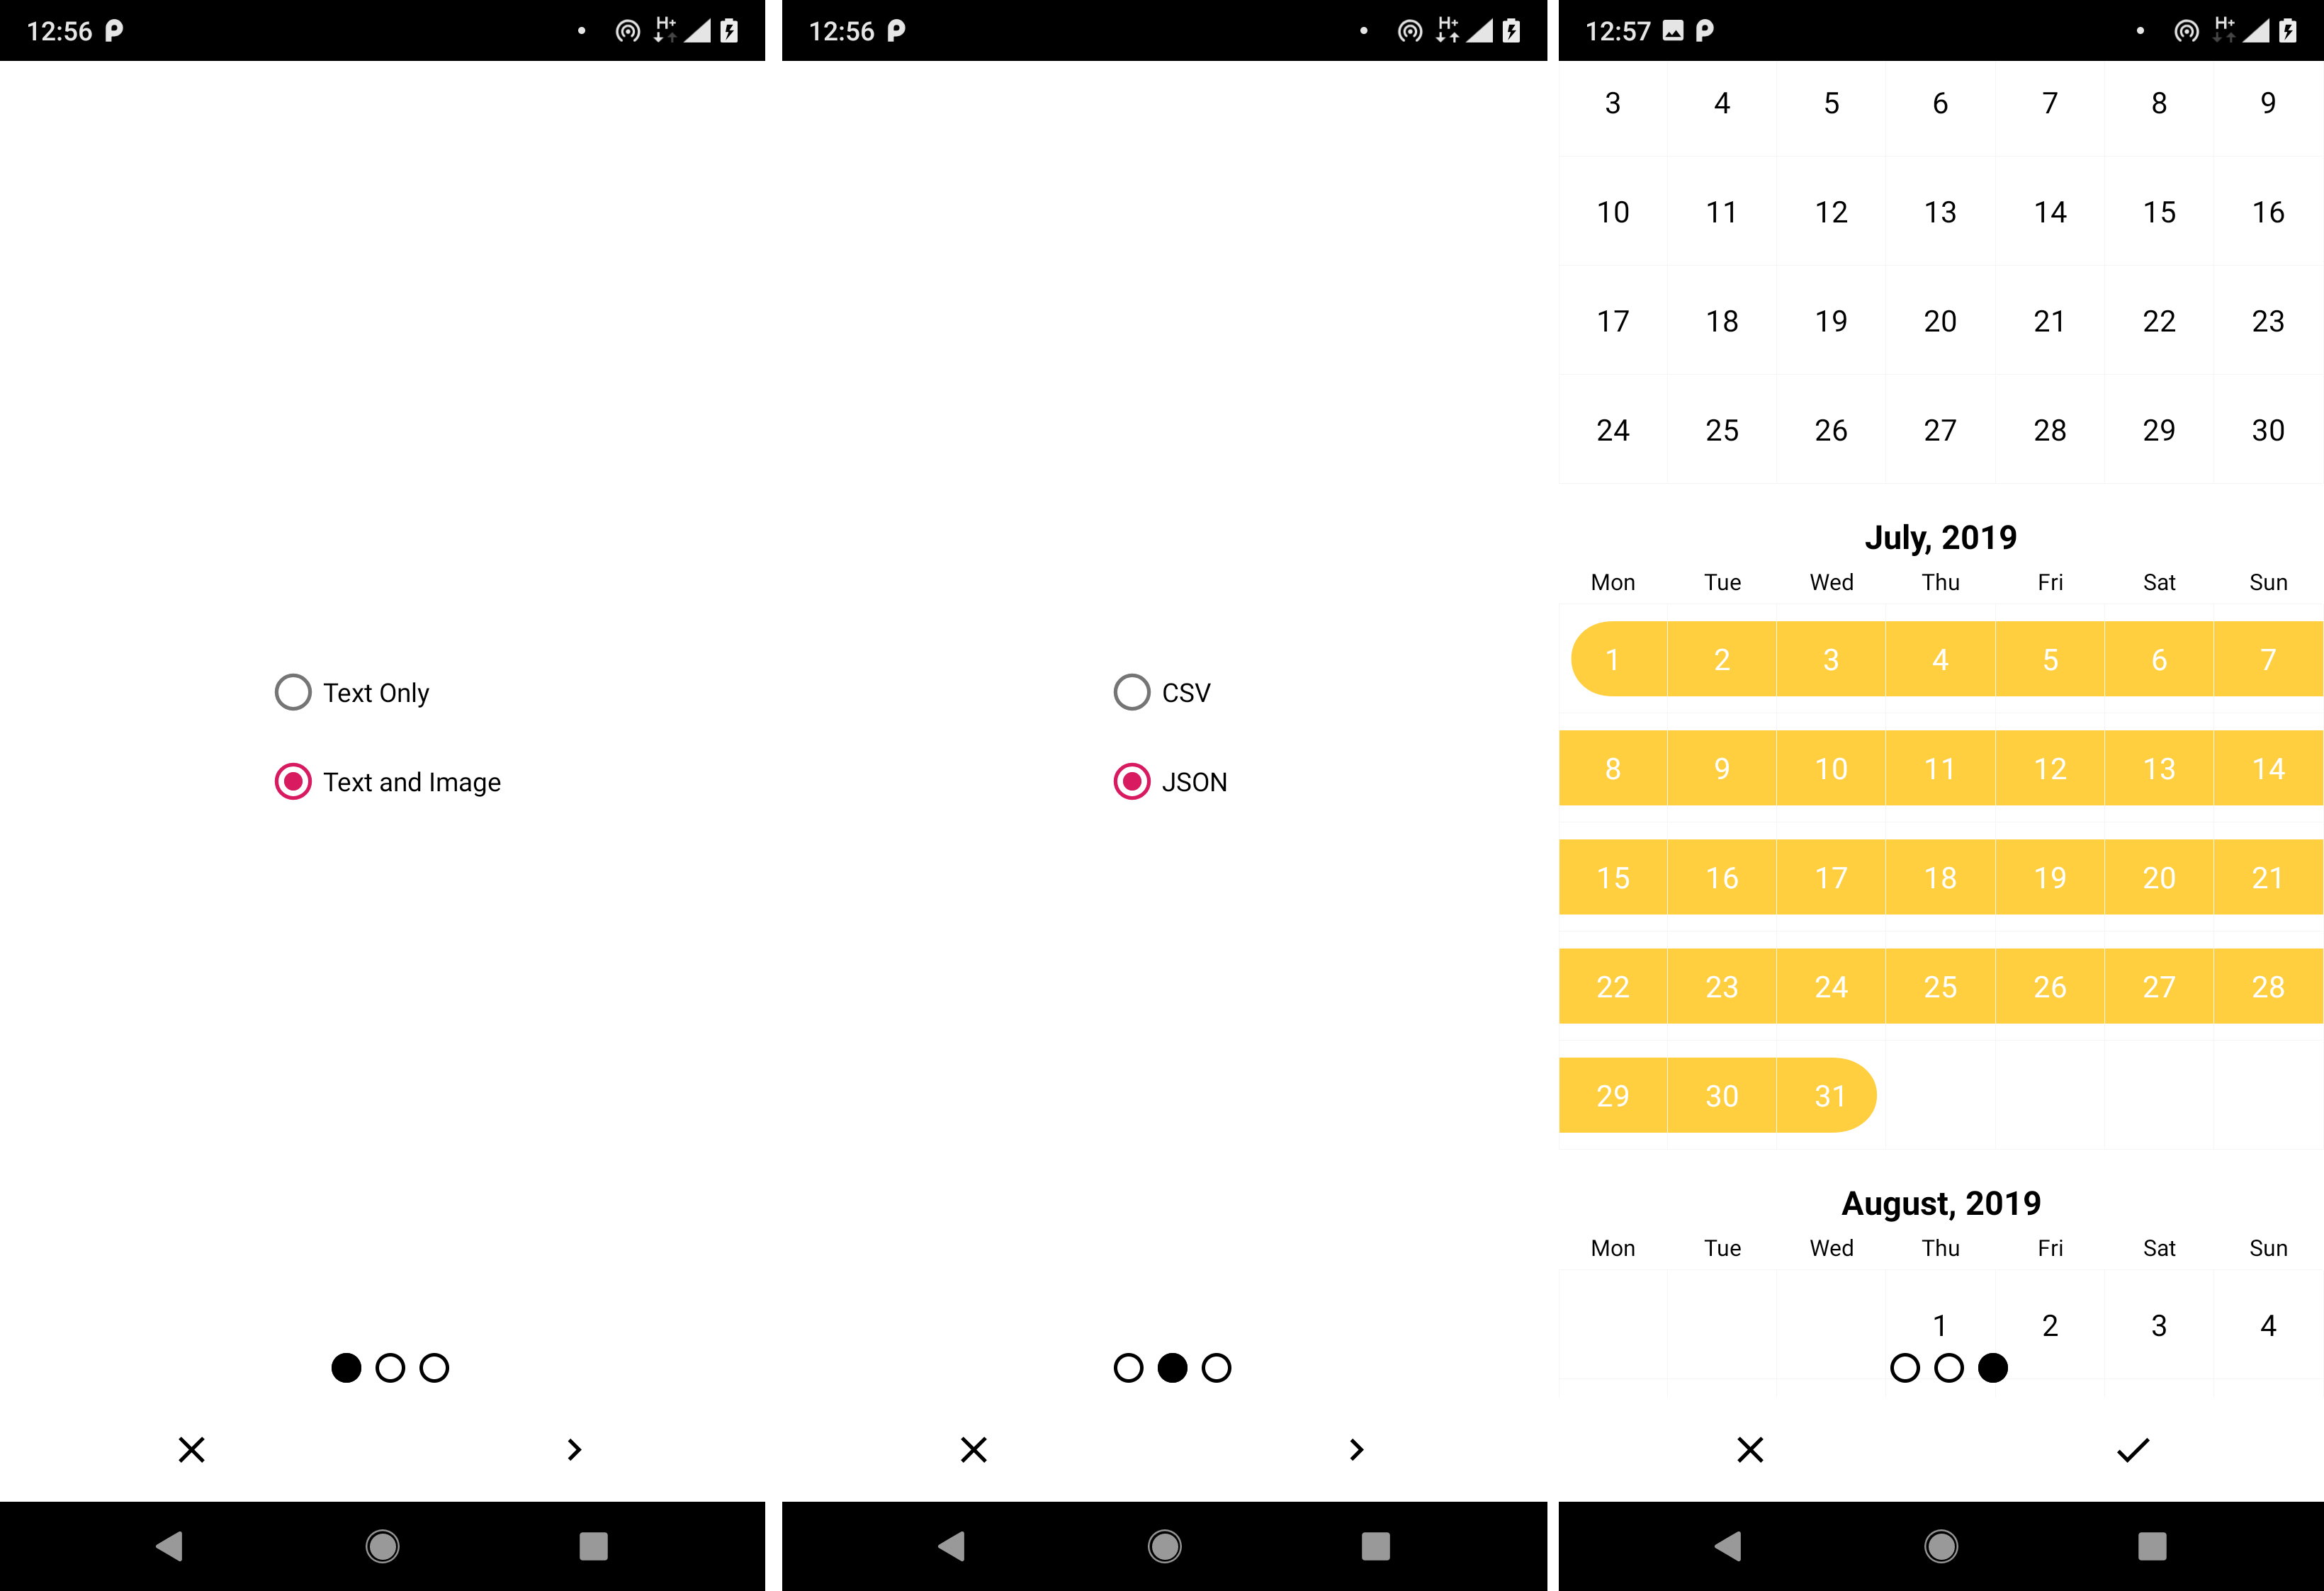
\includegraphics[width=0.95\textwidth]{ExportForm.png}
  \caption{Formularul de export}
  \label{fig:exportForm}
\end{figure}

Odată finalizat exportul datelor, dispozitivul primește o notificare ce conține \emph{link-ul} de descărcare a acestora. Figura \ref{fig:exportsScreen} prezintă ecranul ce afișează lista tuturor \emph{export-urilor} făcute de pe dispozitiv, iar cele complete pun la dispoziție două butoane pentru copierea \emph{link-ului} pe \emph{clipboard}, respectiv descărcarea arhivei.

\begin{figure}[ht]
  \centering
  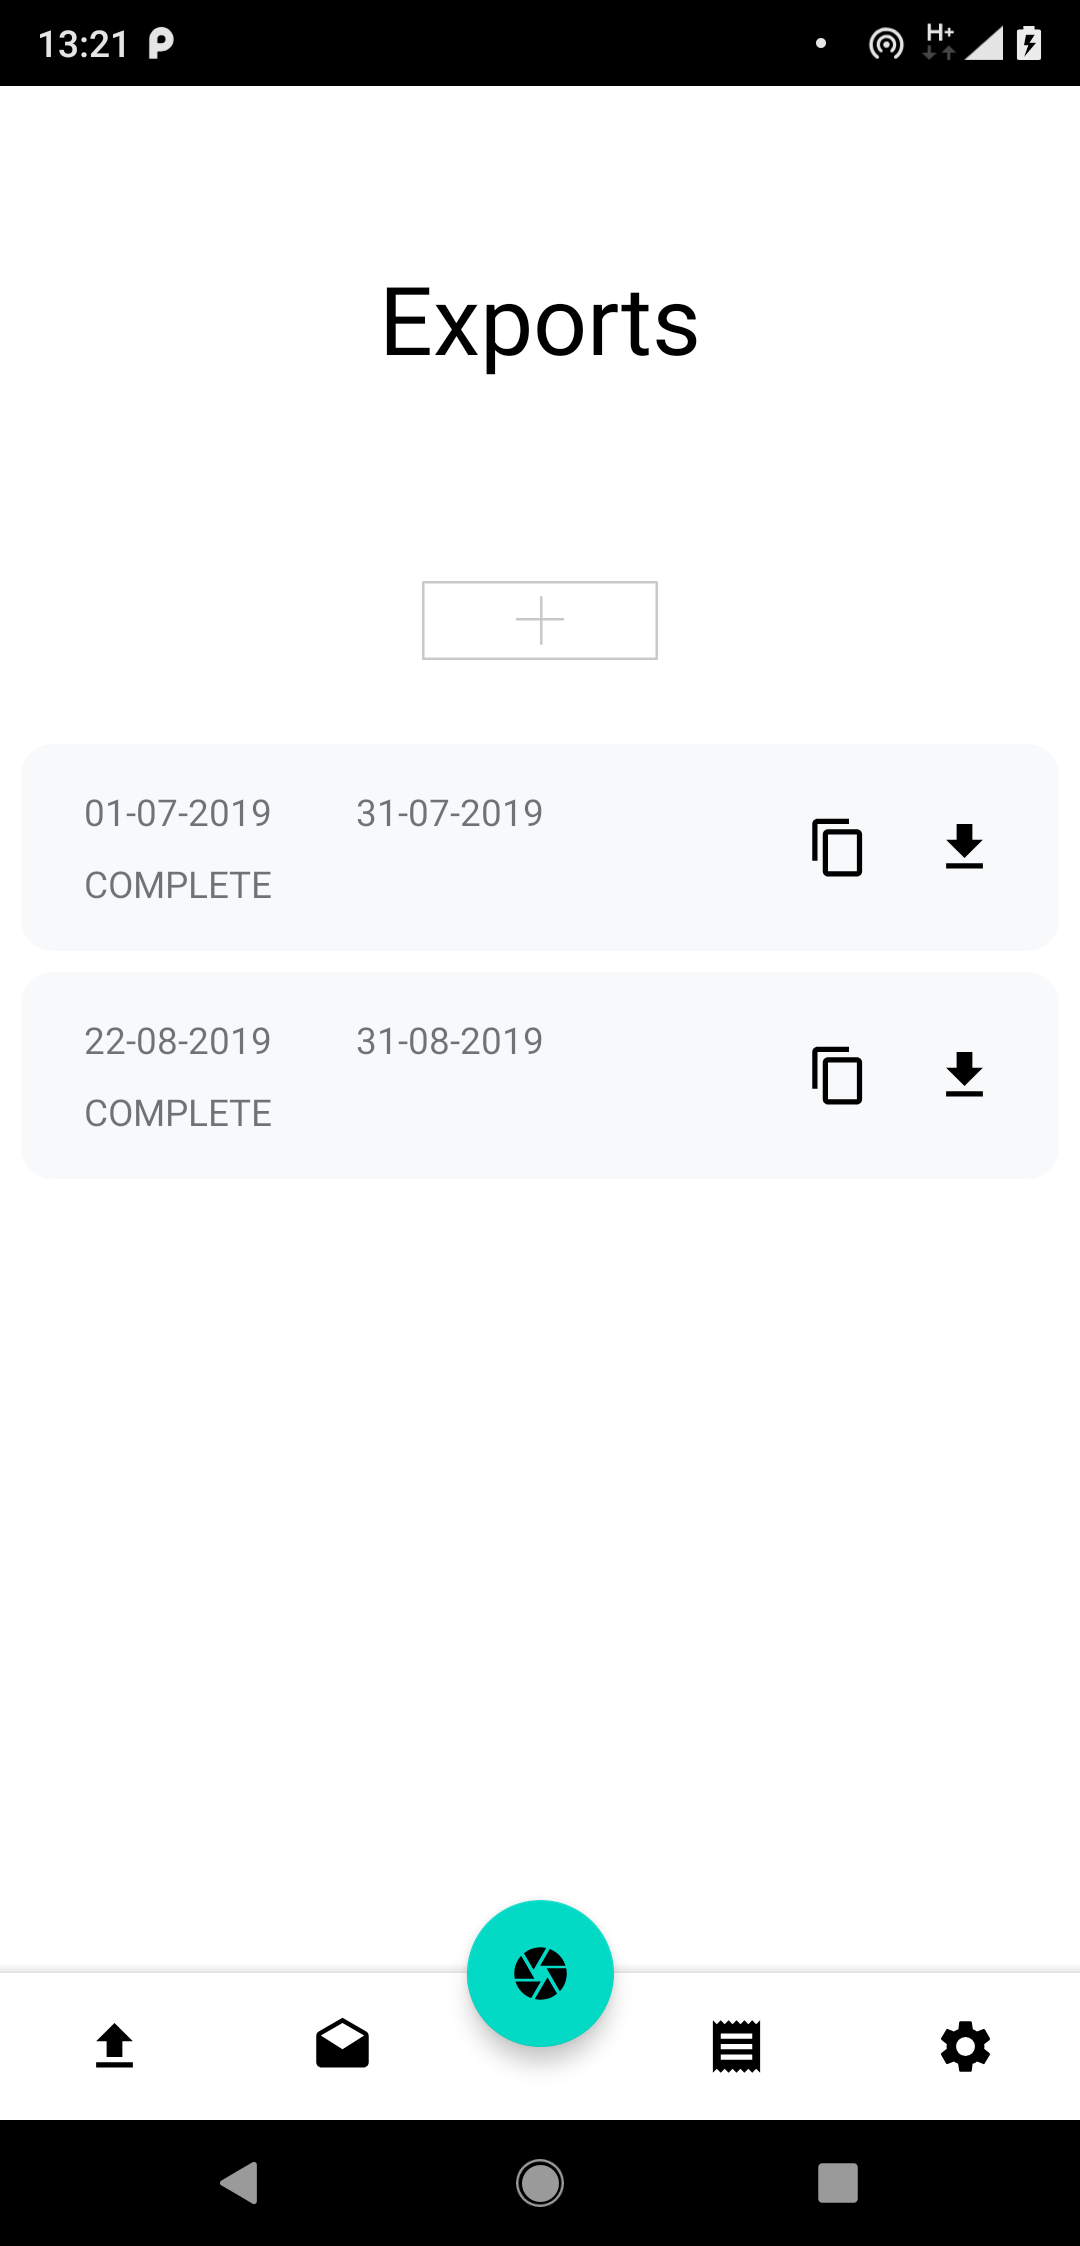
\includegraphics[width=\screenwidth]{ExportsScreen.png}
  \caption{Lista de export-uri}
  \label{fig:exportsScreen}
\end{figure}

\begin{itemize}
\item
  \textbf{Scop}: Accesarea datelor în afara aplicației și a dispozitivului;
\item
  \textbf{Condiție de succes}: Utilizatorul selectează formatul, conținutul și perioada pentru export și primește un link la care poate accesa datele;
\item
  \textbf{Condiție de eșec}: Nu există date înregistrate în perioada selectată; Datele nu sunt trimise cu succes; Utilizatorul nu primește link-ul aferent;
\end{itemize}

\begin{minipage}[t]{0.4\textwidth}

\subsection*{Mențiuni}\label{menux21biuni-3}

\begin{itemize}
  \item
  Pentru a consuma cât mai puține resurse (timp, baterie), exportul se face cu minim de procesare pe dispozitiv;
  \item
  Datele salvate pe cloud au o dată de expirare, după care sunt șterse;
  \item
  Odată ce datele sunt încărcate și procesate în cloud, aplicația primește o notificare ce conține link-ul de descărcare;
  \item
  Datele pot fi descărcate într-o arhivă zip;
\end{itemize}

\end{minipage}\hspace{0.05\textwidth}
\begin{minipage}[t]{0.55\textwidth}

\subsection*{Variații}\label{variaux21bii-2}

\begin{itemize}
\item
  Pentru a oferi maximum de flexibilitate utilizatorilor, datele pot fi accesate în format JSON sau CSV și pot conține fie doar text, fie text și imagini;
\end{itemize}

\subsection*{Extensii}\label{extensii-2}

\begin{itemize}
\item
  În cazul lipsei de conectivitate, acțiunea de export este programată pentru o dată ulterioară, odată ce telefonul are conexiune;
\item
  Toate sesiunile de export sunt înregistrare într-o listă și sunt eliminate odată ce datele aferente sunt șterse din cloud;
\end{itemize}

\end{minipage}



